
\infolevone{\part{Hall A OSP Overview}}
\infoleveqnull{
\chapter{Hall A Specific Safety Information}

\section{Overview}

        The following Hall A subsystems are considered part of the experimental endstation base equipment. 
Many of these subsystems impose similar hazards, such as those induced by magnets and magnet power supplies, 
high voltage systems and cryogenic systems.  Note that a specific sub-system may have many different hazards associated with it.

The material in this chapter is a subset of the material in the full Hall A operations manual and is only intended to familiarize
people with the hazards and responsible personnel for these systems.  It in no way should be taken as sufficent information to
use or operate this equipment.
}

\graphicspath{{introduction/figs/}}
\renewcommand{\dirfig}[0]{introduction/figs}
\renewcommand{\dircur}[0]{introduction}

%\chapter{Introduction}
\chapter[Introduction]{Introduction
\footnote{
  $CVS~revision~ $Id: a-intro.tex,v 1.3 2003/12/05 07:23:23 gen Exp $ $ 
}
\footnote{Authors: J.LeRose \url{mailto:lerose@jlab.org} and
                   E.Chudakov \url{mailto:gen@jlab.org}}
}
\ifpdfhref{ 
\section[About this Document]{Technical Information About this Document}
\label{sec:intro-about}
 {\it
 This is a PDF document with hyper-references. Browsing is helped
 by the ``bookmark'' menu at the left side of the \mycomp{acroread}
 window. Another browser, \mycomp{xpdf} seems to lack this option.
 The objects like
 citations, figures, tables etc. are hyper-marked. One can ``click''
 on a reference to an object and jump to the page with this
 object. Jumping back can be done using the right mouse button (\mycomp{acroread})
 or the left arrow button at the bottom of the window (\mycomp{xpdf}).
 External references to the Web are also ``clickable''.
 In order to use them, make sure that your PDF browser is configured
 to work with a Web browser (use the button ``Preferences'' in \mycomp{acroread},
 or provide and edit the file \mycomp{$\tilde{}$/.xpdfrc} for \mycomp{xpdf}).
 One should open a Web browser window and afterward one may
 use the WWW-links from the PDF browser. Finally, the PDF browsers
 allow to search for a given pattern in the whole document. 

 The areas of text, dedicated to
 safety issues, are marked by red color throughout this document.
 Sometimes only the titles of the appropriate sections are marked. 
 
 \LaTeX{} (more specifically, \mycomp{pdflatex}) is used to produce
 this document. The document source is kept in CVS~\cite{CVSwww} format\footnote{
   Instruction for the document authors/maintainers: 
   \url{http://www.jlab.org/~gen/osp/doc.pdf}.}.

 Typically, each chapter or a big section occupies one file,
 and the date of CVS revision of the file is printed
 in a footnote for the chapter title. \\

 This document can be printed, but it is better used on-line.
}
\clearpage
}

\section[Purpose]{The Purpose of this Document}
\label{sec:intro-purpose}

 This document contains the following information concerning the Hall
 A ``base equipment'':
 \begin{list}{--}{\setlength{\itemsep}{-0.2cm}}
    \item general overview; 
    \item safety assessment; 
    \infolevone{\item technical overview;} 
    \infolevtwo{\item operating procedures;} 
    \infolevthree{\item performance information.}
 \end{list}

\noindent{}The requirements to Hall A personnel training 
are outlined in Sec.~\ref{sec:access-req}. 
Although reading of this OSP document is not explicitly required, 
the other documents refer to it, as far as
safe operations of the base Hall A equipment are concerned.\\

\infolevtwo{
  The operating procedures are intended to
  provide shift personnel with the information they need to
  understand, at least at a rudimentary level, the function of the
  various subsystems in the end-station. It should also aid in
  determining if the equipment is performing properly and provide
  instructions for what to do in the case of malfunctions. This
  document does not necessary give a complete comprehensive reference 
  to each subsystem, but at least provides a guide for the shift 
  personnel. When appropriate,
  other references are indicated for the user who requires more
  information.  \\
}

 A comprehensive description of the equipment performance in given
 in a published paper~\cite{HallA-NIM}. 
\infolevtwo{
 This OSP includes some
 information on this matter in order to help the shift workers
 to check up the equipment.
}

\infolevltthree{
\begin{safetyen}{10}{15}
 This is a reduced version ({\it ``info level \infolevel{}''}) of the OSP document. 
 It is sufficient to get acquainted with the base equipment but might be not
 sufficient to operate it. For operation one should read the
 full ({\it ``info level 4''}) OSP document~\cite{HallAosp}.  
\end{safetyen}
}
\clearpage
\section[Hall A Overview]{Hall A Overview}
\label{sec:intro-halla-overview}

The design purpose of Hall A is to study electron scattering 
on nuclei and nucleons at high luminosity
of up to $5\cdot{}10^{38}~\mathrm{cm^{-2}s^{-1}}$ with high momentum
resolution. The ($e,e^{\prime}p$) reaction is often utilized.
The spectrometers must have high resolution 
to be able to isolate the different reaction channels in nuclei.

The basic lay-out of Hall A is shown in Fig.~\ref{fig:HallA-side},
demonstrating the Hall dimensions.
\infolevtwo{A CAD-drawn 3-dimensional view of the Hall 
is given on the scalable picture on the \hyperlink{pict:cover}{cover} page.}

\begin{figure}[htb]
 \begin{center}
    \includegraphics*[angle=0,width=\textwidth]{HallA}
 \end{center}
\caption[Hall A schematic cross section]%
{Schematic cross section of Hall A with one of the HRS 
spectrometers in the (fictitious) 0$^\circ$ position. 
}
\label{fig:HallA-side}
\end{figure}

The beam line transports the CEBAF electron beam, in the energy 
and current ranges of 0.8~-~6.0~GeV and 0.1~-~120~$\mu$A to the target
at the Hall center. Various types of targets have been used, including
liquid hydrogen and polarized $^3$He gas. Secondary particles
are detected with the  
two High Resolution Spectrometers (HRS). Both of these devices  
provide a momentum resolution of better than $2\times 10^{-4}$ and a horizontal angular 
resolution of better than 2 mrad at a design maximum central momentum 
of 4 GeV/$c$. The rest of the beam is transported to the high power
water cooled beam dump.

The present base instrumentation in Hall A has been used with great 
success for experiments which require high luminosity and high resolution 
in momentum and/or angle for at least one of the reaction products.
	
%\infolevthree{  
%  A CAD-drawn view of Hall A and its basic equipment is shown
%  on Fig.\ref{fig:cad_halla_1}.
%\begin{figure}[tbh]
%\begin{center}
%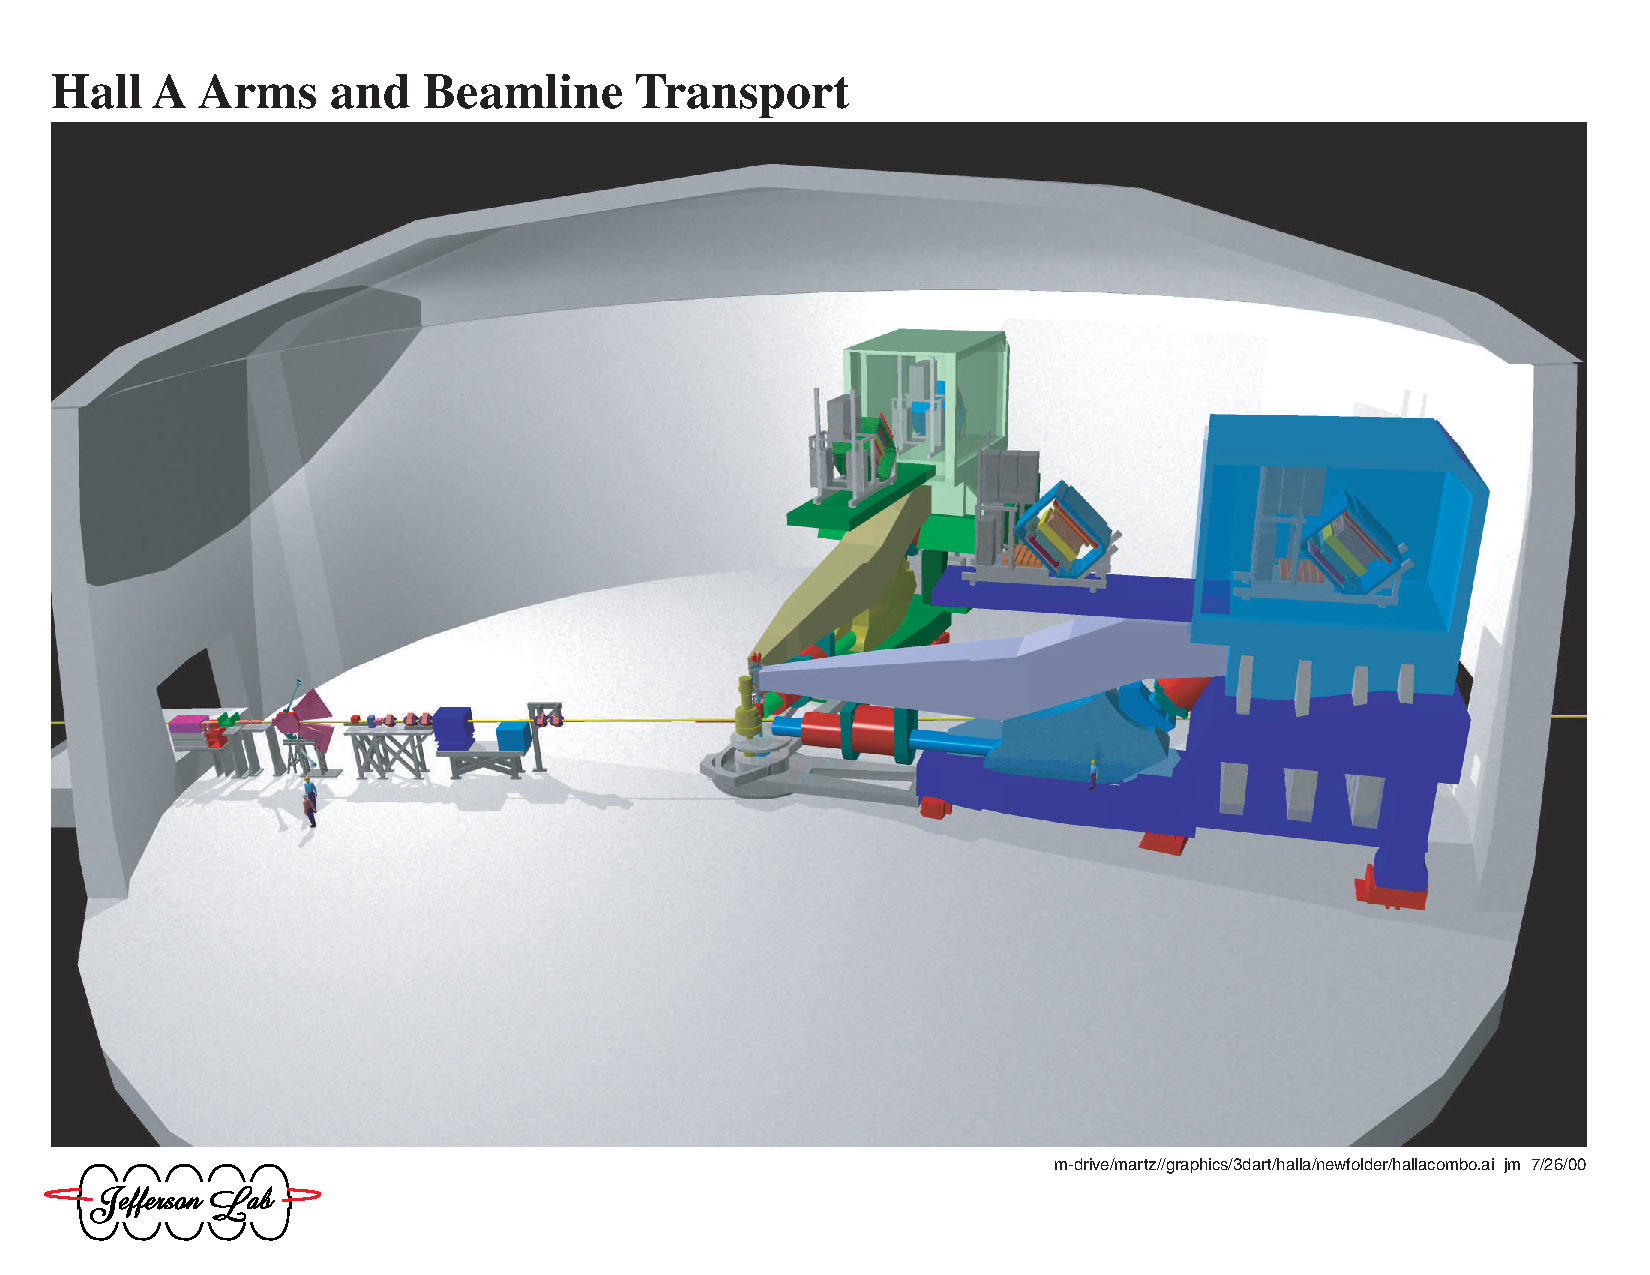
\includegraphics[angle=0,width=\textwidth]{hallacombo}
%\caption[Hall A CAD-drawn picture]
%   {Hall A CAD-drawn picture.}
%\label{fig:cad_halla_1}
%\end{center}
%\end{figure}
%}
% ===========  CVS info
% $Header: /group/halla/analysis/cvs/tex/osp/src/introduction/a-intro.tex,v 1.3 2003/12/05 07:23:23 gen Exp $
% $Id: a-intro.tex,v 1.3 2003/12/05 07:23:23 gen Exp $
% $Author: gen $
% $Date: 2003/12/05 07:23:23 $
% $Name:  $
% $Locker:  $
% $Log: a-intro.tex,v $
% Revision 1.3  2003/12/05 07:23:23  gen
% Many modifications in the introduction, new pictures
%
% Revision 1.1  2003/06/06 15:26:26  gen
% Revision printout changed
%
% Revision 1.3  2003/06/06 14:36:44  gen
% Revision printout changed
%
% Revision 1.2  2003/06/05 23:30:01  gen
% Revision ID is printed in TeX
%
% Revision 1.1.1.1  2003/06/05 17:28:28  gen
% Imported from /home/gen/tex/OSP
%
%  Revision parameters to appear on the output


\infolevone{\chapter[Hall A Safety Assessment Overview]{Hall A Safety Assessment Overview
%\section[General]{General
\footnote{
  $CVS~revision~ $Id: sad-overview.tex,v 1.1 2005/04/04 22:27:25 gen Exp $ $ 
}
\footnote{Authors: E.Chudakov \email{gen@jlab.org}, based on an old ESAD}
}
 
\begin{safetyen}{10}{15}
\section{Overview of the Hazards} 
\end{safetyen}
\label{sec:overviewhazards}

The purpose of this section is to give a general overview of the hazards one may encounter
while in Hall A,
without going into the details of each part of the equipment. In order to 
be able to operate a particular piece of equipment in a safe way one must study the appropriate
section of  
\infolevltthree{the full OSP manual\cite{HallAosp}.}
\infolevthree{this OSP manual.}
The general hazards are:
\begin{list}{\arabic{enumi}.~}{\usecounter{enumi}\setlength{\itemsep}{-0.15cm}}
  \item Radiation hazard (see Sec.\ref{sec:radhazard});
  \item Fire hazard (see Sec.\ref{sec:firehazard});
  \item Electrical hazard (see Sec.\ref{sec:electrhazard});
  \item Mechanical hazard (see Sec.\ref{sec:mechhazard});
  \item Hazard from strong magnetic fields (see Sec.\ref{sec:maghazard});
  \item Cryogenic and Oxygen Deficiency Hazard (ODH) (see Sec.\ref{sec:odhhazard});
  \item Vacuum and high pressure hazards  (see Sec.\ref{sec:vachazard});
  \item Toxic materials hazard  (see Sec.\ref{sec:toxichazard}).
\end{list}

The principal contacts for Hall A safety issues are given in Tab.\ref{tab:ehs:principlecont}.
 
\begin{namestab}{tab:ehs:principlecont}{Principle contacts for safety issues}{%
   Principle contacts for safety issues}
  \EdFolts{\em Safety Warden}
  \BertManzlak{\em EHS Engineer}
\end{namestab}
 
\begin{safetyen}{0}{0}
\section{Radiation Hazard} 
\label{sec:radhazard}
\end{safetyen}
  The radiation hazards and the ways to mitigate them are described in detail in the
  course of Radiation Worker I (RW-I) training~\cite{RWIcebaf},
  as well as in the Hall A Radiation Work Permit (RWP).
  Here, the most essential issues are discussed.

  CEBAF's high intensity, high energy electron beam 
  is a potentially lethal radiation source and hence many redundant measures,
  called Personnel Safety System or PSS~\cite{PSScebaf}, are in place,
   aimed at preventing accidental exposure of personnel to the beam or exposure 
  to beam-associated radiation sources.
  The PSS keeps ionizing radiation out of areas where people are working,
  and keeps people out of areas where ionizing radiation is present. 
  The PSS procedure to enter the hall is described in detail in  Sec.~\ref{sec:Access}.

%  Here, we remind of a few items.

% \begin{list}{--}{\setlength{\itemsep}{-0.cm}}
%    \item 
 All of Hall A is qualified as a ``Radiologically Controlled Area''~\cite{RWIcebaf}.
 Entrance requirements are listed in Sec.\ref{sec:access-req}.
 Some areas, such as the target area, and the area around the beam dump may be qualified as 
 a ``Radiation Area'' or a ``High Radiation Area''. Some areas may be also qualified 
 as a ``Contaminated Area', if removable radio-isotopes are likely to be present.
 These areas should be marked with appropriate signs and may be delimited by barrier. 
 Access to ``Radiation Areas'' requires a permit from RadCon, while access
 to ``High Radiation Area'', and ``Contaminated Area'', is not allowed. One should consult 
 the RWP document for more details.

 All the items, except those kept in the shielded detector huts of HRS,
          which stayed in the Hall during CW beam operations,
          must be surveyed and released by a qualified Radiological Control Technologist from
          RadCon group, prior to removal from the hall.
          A rack close to the entrance is used to store these items.

 Some electronic modules and racks are posted as potentially contaminated.
 They must be surveyed and, if necessary, cleaned by RadCon personnel,
 prior to removal from the Hall, or prior to performing any work on the internal parts of the racks
 and modules, including the air filters. 
 
 More details on radiation safety issues can be found in various sections of this 
 document, as in Chap.\ref{sec:targets-overv} for target operations and
 in Sec.\ref{sec:beam-intro} for operation of the equipment on the beam line.
 
 The contacts for Hall A radiation safety issues are given in Tab.\ref{tab:ehs:radiation}.
 
 \begin{namestab}{tab:ehs:radiation}{Contacts for radiation safety issues}{%
   Contacts for radiation safety issues}
  \EdFolts{\em Safety Warden}
  \RadCon{\em RC Group}
 \end{namestab}


\begin{safetyen}{0}{0}
\section{Fire Hazard} 
\label{sec:firehazard}
\end{safetyen}

 Fire Hazards are associated with the use of electrical power and also with the use of 
 flammable gases and/or materials. 

 The flammable gasses include the cryotarget
 materials such as hydrogen or deuterium 
 (see the details on the hazard and its mitigation in Sec.\ref{sec:target-cryo-safety}) as well as
 the gas used in the wire detectors of the spectrometers 
 (see the details on the hazard and its mitigation in Sec.\ref{sec:hrs-det-gasalarms}).
 
 In general an effort has been made to limit the volume of combustible material 
 in the hall but some flammable material is unavoidable. For instance all plastic 
 scintillators are flammable and if exposed to a direct flame these 
 plastic materials will eventually melt. The elements then lose structural integrity, 
 sag or fall to the floor, and the melted elements would likely be exposed to air and burn.

 Some special equipment in the subsystems, like heaters, lasers etc., may present a
 fire hazard (see Sec.\ref{sec:targ-polhelfire}\infolevone{ and Sec.\ref{sec:heaterinterlock}}).
 
 The fire hazard in Hall A is mitigated by a VESDA smoke detection system. 
% The head sensitivity of 
% the VESDA is 0.03 to 0.003\%. This corresponds to approximately 1 % of full scale and the system trips 
% at 90\% full scale. 
 The main VESDA panel is located in the room at the bottom of the truck ramp on the 
 right hand side as you walk out of Hall A. The clean power in the detector huts is 
 interlocked to the VESDA system. If the VESDA system senses smoke, it will remove power 
 from the huts.

 The detector huts are equipped with a clean agent fire suppression system. This system, when triggered 
 by a smoke detector installed on the hut ceiling, releases an inert gas mixture into the hut and dilute
 s the oxygen level below that needed to sustain combustion. The inert gas is a mixture of nitrogen, 
 argon and carbon dioxide. When the system is functioning properly the oxygen content of the air in the 
 hut will be reduced to approximately 12.5\% from the standard 21\%. Operation of this system
 would result in an ODH hazard (see Sec.\ref{sec:odhhazard}).

 In case of a fire alarm personnel should leave the area. Upon seeing a fire
 or unexplained smoke one should activate the fire alarm, leave the area and
 call 911 and 4444 from a safe place (see \cite{EHScebaf}).
  
 The contacts for Hall A fire safety issues are given in Tab.\ref{tab:ehs:fire}.
 
 \begin{namestab}{tab:ehs:fire}{Contacts for radiation safety issues}{%
   Contacts for radiation safety issues}
  \EdFolts{\em Safety Warden}
  \BertManzlak{\em EHS Engineer}
 \end{namestab}

\begin{safetyen}{0}{0}
\section{Electrical Hazard} 
\label{sec:electrhazard}
\end{safetyen}

 Almost every subsystem in Hall A requires AC and/or DC power. Due to the high current
 and/or high voltage requirements of many of these subsystems the power supplies providing this 
 power are potentially lethal.

 Aside from the resetting of a small branch circuit breaker you should not attempt to solve
 any other problems associated with AC power distribution without consulting responsible personnel. All
 the power distribution boxes are clearly marked to aid in finding the appropriate circuit breaker in
 the event of a problem.

 There is a ``Hall A power'' crash button in the counting house. This is intended for dire emergency use. 
 It is possible to cause severe damage to Hall A systems (in particular the hadron spectrometer dipole) 
 by inappropriate use of this power kill switch.

 Anyone working on AC power in Hall A must be familiar with the EH\&S\cite{EHScebaf} manual 
 and must contact one of the responsible personnel. Lock and Tag training may also be required.

 The DC power supplies energizing the magnets can provide a very high current.
 There is a danger of metal tools coming into contact with exposed leads, shorting out the
 leads, depositing a large amount of power in the tool, vaporizing the metal, and creating an arc.
 These hazards are mitigated by covers installed around the leads,
 preventing accidental access to them. The covers must not be removed
 unless the magnet is turned off using the Lock and Tag procedure by trained
 personnel. 

 The electronics NIM, CAMAC, FASTBUS and VME crates are equipped with high current
 DC power supplies for $\pm$5~V and other low voltages. Although their power 
 is typically lower than the power supplied for magnets,
 care should be taken to avoid accidental contact to the leads with metal tools.
 Typically, covers are installed on the back of the crates or the racks,
 in order to mitigate the hazard. 

 Another electrical hazard is caused by high voltage (HV) in a range of 1-3~kV  DC power used 
 for photomultiplier tubes. The current per channel, provided by the appropriate power supplies,
 is limited to about 1-2~mA. 
 The HRS detectors 
 (see Sec.\ref{chap:hrs-det}), as well as the beam line equipment use 
 hundreds of such channels. 
 Typically, the power is provided through special cables (of red color). The cables and SHV connectors 
 meet the existing EH\&S standards. Even with the cables disconnected, an accidental
 contact with the power electrodes is not probable. In order to avoid the hazard to the personnel
 as well as damage to the equipment, one should not attach/remove HV cables or the
 phototube bases when HV is present on a given channel. Formally, the ``Lock out / Tag out'' 
 procedure is not required to operate this equipment. However, turning the HV off
 and making sure that it is not accidentally turned on remotely or locally, is required.
 The LeCroy~1458 power supply mainframes, used in Hall A, are equipped with
 a control key on the front panel. The key should be turned to ``local'' mode in order to
 avoid remote operation. If the power supply is located far from the working place,
 it is recommended that the crate be turned off and the key be removed.
 
 Numerous cables, including HV cables and high current cables, are installed in trays, 
 racks and other accessible areas. Damage to these cables may result
 in hazards to personnel and equipment. 

 The contacts for Hall A electrical safety issues are given in Tab.\ref{tab:ehs:electrical}.
 
 \begin{namestab}{tab:ehs:electrical}{Contacts for radiation safety issues}{%
   Contacts for radiation safety issues}
  \EdFolts{\em Safety Warden}
  \MarkStevens{}
 \end{namestab}

 
\begin{safetyen}{0}{0}
\section{Mechanical Hazard} 
\label{sec:mechhazard}
\end{safetyen}

 One source of mechanical hazards includes the heavy movable 
 elements in Hall A, as the HRS~\ref{sec:hrs-safety} and the detector hut doors.
 In order to alert personnel, visible and audible signals are issued when
 the spectrometers or the doors are moving.   
 The HRS motion can be controlled remotely from the counting house,
 in the angular range $>15^\circ$. Motion at smaller angles
 must be performed by the hall technicians only (see \ref{tab:ehs:mechanical}).
 Since motion at large angles may be hindered by equipment stored on the floor,
 Ed Folts provides ``administrative limits'' for spectrometer motion for
 the current time period. Typically, the safe limits for the HRS motion 
 are enforced by pins planted in the hall floor, however the shift crews should
 be aware of the current limits and never exceed them.

 There are conventional
 hazards like fall hazards and crane hazards. The installed safe ladders and hand rails
 mitigate the fall hazards. Working on elevated areas beyond the hand rail protection
 requires the use of safety harnesses or other means. One should consult the contact
 personnel (see Table\ref{tab:ehs:mechanical}) before starting such a work.
 The safety of crane operations is supervised by the hall technical staff. 

 The contacts for Hall A mechanical safety issues are given in Tab.\ref{tab:ehs:mechanical}.
 
 \begin{namestab}{tab:ehs:mechanical}{Contacts for mechanical safety issues}{%
   Contacts for mechanical safety issues}
  \EdFolts{\em Safety Warden}
  \MarkStevens{}
 \end{namestab}

 
\begin{safetyen}{0}{0}
\section{Hazard from Strong Magnetic Fields} 
\label{sec:maghazard}
\end{safetyen}

 Personnel working in the proximity of the energized, strong  magnets of the HRS or the beam line
 are exposed to the following magnetic hazards:
 \begin{list}{--}{\setlength{\itemsep}{-0.cm}}
    \item electrical hazards, described in Sec.\ref{sec:electrhazard};
    \item danger of magnetic objects being attracted by the magnet fringe field, and becoming airborne;
    \item  danger of cardiac pacemakers or other electronic medical devices no longer
           functioning properly in the presence of magnetic fields;
    \item danger of metallic medical implants (non-electronic) being adversely affected
          by magnetic fields.
 \end{list}

 Several measures are taken to mitigate the hazards. 
 Whenever a magnet is energized, a flashing red light on the magnet or on the
 magnet support structure is activated to notify and warn personnel of 
 the associated electrical and magnetic field hazards.
 
 Administrative measures are implemented to
 reduce the danger of magnetic objects being attracted by the magnet 
 fringe field and becoming airborne. (Note that for most magnets strong magnetic 
 fields are only encountered within non-accessible areas inside the magnet.) 
 Areas where these measures are in effect are clearly marked.

 To reduce the danger of magnetic fields to people using pacemakers or other medical
 implants, warning signs are prominently displayed at the entrance to the hall. 

 The contacts for Hall A magnetic safety issues are given in Tab.\ref{tab:ehs:magnetic}.
 
 \begin{namestab}{tab:ehs:magnetic}{Contacts for mechanical safety issues}{%
   Contacts for mechanical safety issues}
  \EdFolts{\em Safety Warden}
 \end{namestab}

\begin{safetyen}{0}{0}
\section{Cryogenic and Oxygen Deficiency Hazard (ODH)} 
\label{sec:odhhazard}
\end{safetyen}

The superconducting magnets are all operated at temperatures of about 4~K. 
This temperature is obtained by refrigeration with liquid (or super critical) 
helium supplied from the End Station Refrigerator (ESR).

During normal operation the superconducting magnets consume $\sim$14~g/s of Helium. 
In addition, the cryostats of these magnets have an inventory of liquid Helium. If a magnet ``goes
normal'' for whatever reason this Helium inventory will be rapidly boiled. Relief systems have been 
installed on the magnets to protect the vessels from building undue pressures during a quench event. 
However, all superconducting magnets are at least somewhat subject to damage in the event of a quench. 
The magnets have quench protection circuitry designed to safely dispose of the magnets 
stored electromagnetic energy.

Contact with cryogenic fluids presents the possibility of severe burns (frostbite). 
When handling these fluids, Liquid Nitrogen or Helium, one must follow the
guidelines in the EH\&S manual\cite{EHScebaf}. These guidelines mandate the use 
of cryogenic gloves and eye protection.

All volumes in the cryogenic systems which can be isolated by valves or any other 
means are equipped with pressure relief valves to prevent explosion hazards.
The release and subsequent expansion of cryogenic fluids presents the possibility 
of an oxygen deficiency hazard. Rapid expansion of a cryogenic fluid in a confined 
space presents an explosion hazard. Cryogenics in Hall A are present in the superconducting 
HRS magnets, and the scattering chamber with its cryogenic targets. The total 
inventory of cryogens in the magnets and targets present a minimal ODH hazard in all 
areas of the hall except the area above the Hall A crane\infolevone{ (see also Sec.\ref{sec:targ:odh})}.

There are a number of vessels which are normally filled with oxygen free atmosphere. 
These include the gas Cerenkov, the spectrometer vacuum space and the scattering chamber. 
Service of these vessels could represent a ODH (confined space) hazard.

Hall A is listed as an Oxygen Deficiency Hazard area of Class 0. 
No unescorted access is allowed without up-to-date JLab ODH training.

No one should enter the Cerenkov tanks while there is gas inside these tanks. 
The tanks should be pumped out and filled with air before access to the interior 
of these tanks is permitted. 
The HRS detector huts may present an ODH hazard in case of the fire suppression 
system activation (see Sec.\ref{sec:firehazard}), if the doors of the hut are shut. 
No one may stay in the hut with the doors shut.
  
 The contacts for Hall A cryo and ODH safety issues are given in Tab.\ref{tab:ehs:cryo}.
 
 \begin{namestab}{tab:ehs:cryo}{Contacts for cryogenic safety and ODH issues}{%
   Contacts for cryogenic safety and ODH issues}
  \BertManzlak{\em EHS Engineer}
  \EdFolts{\em Safety Warden}
 \end{namestab}

\begin{safetyen}{0}{0}
\section{Vacuum and High Pressure Hazards} 
\label{sec:vachazard}
\end{safetyen}

The greatest safety concern for the vacuum vessels in use in Hall A are the thin 
aluminum, titanium or kapton windows that close the entrance and/or exit of 
these vessels. The HRS spectrometer vacuum vessel, and the Hall A Scattering Chamber 
both contain thin windows.

The HRS Vacuum System is described in detail in Chapter~\ref{chap:vacuum}. 
The space between the magnet poles of both spectrometers is evacuated in order 
to diminish multiple scattering. The entrance and exits of the main spectrometer 
volumes are covered by relatively thin vacuum windows. 
The vacuum safety of the cryo-target is described in Sec.\ref{sec:target-cryo-safety}. 

The HRS spectrometer vacuum can has a volume of approximately 6 m$^3$.
%, representing a stored energy of 6 \Theta  105 Joules. 
The circular (7 inch diameter) entrance window on the front of Q1 is made of 0.007~inch thick 
kapton while the rectangular 90.89" by 6.41" exit window located in the shield hut below the VDC 
is 0.004~inch thick Ti (3,2.5) Alloy. The scattering chamber contains two windows 
constructed from 0.016~inch thick 5052 aluminum.

Installation of vacuum windows can only be done by the responsible personnel following
detailed instructions provided in the Operations Manual.
Before entering the detector huts or pivot area, all personnel should
check the spectrometer and/or scattering chamber vacuum gauges. If the spectrometers 
and/or scattering chamber are under vacuum:
 \begin{list}{--}{\setlength{\itemsep}{-0.cm}}
    \item Use careful judgment if it is necessary to work near the vacuum windows;
    \item Do not work near the windows any longer than is absolutely necessary;
    \item Never touch the vacuum windows, neither with your hands nor with tools;
    \item Do not place objects so that they may fall on the windows, etc.;
    \item Hearing protection is required when working near the target chamber windows and 
          is recommended in the shield huts.
 \end{list}

Window covers must be in place over the target chamber whenever the hall is in
Restricted access. The windows covers must also be employed whenever extensive 
work must be done in the area of the pivot.
Window covers must be placed over the spectrometer exit windows when they are
not covered by the detector package.

The highest gas pressure used in Hall A is about 2000~PSI ($\sim$140~atm) in the bottles
of argon and other gasses used to flush the drift chambers of HRS 
(see Chapter~\ref{chap:hrs-det-gas}). The bottles (``cylinders'') are installed
in a gas shed outside the hall. To ease handling, gas bottle carts are available for use 
in the hall and the gas shed. Typically, the Hall A technicians handle the gas bottles. 
Bottles must never be left free standing. They must always be stored in a rack, 
on a cart or tied to a support.

Polarized $^3$He targets contain Helium gas at $\sim$10~atm in a glass cell.
Hearing protection is mandatory when working near the glass 
cell\infolevone{ (see Sec.\ref{sec:targ-hel-saf})}.   
 
 The contacts for Hall A vacuum and pressure safety issues are given in Tab.\ref{tab:ehs:vacuum}.
 
 \begin{namestab}{tab:ehs:vacuum}{Contacts for vacuum and pressure issues}{%
   Contacts for vacuum and pressure issues}
  \BertManzlak{\em EHS Engineer}
  \EdFolts{\em Safety Warden}
 \end{namestab}

\begin{safetyen}{0}{0}
\section{Toxic Materials Hazard} 
\label{sec:toxichazard}
\end{safetyen}

 Some of our target materials may pose a safety concern. Presently the
 only hazardous target materials used is ceramic Beryllium-Oxide (BeO).
 In solid form, BeO is completely safe under normal conditions of use.
 The product can be safely handled with bare hands. However, in powder form 
 all Beryllia are toxic when airborne. Overexposure to airborne Beryllium particulate 
 may cause a serious lung disease called Chronic Berylliosis. 
% Beryllium has also been listed as a potential cancer hazard. 
% Furthermore exposure to Beryllium may aggravate medical conditions related to 
 airway systems (such as asthma, chronic bronchitis, etc.). 
 Since beryllia are mainly dangerous in powdered form, do not machine, break, or 
 scratch these products. Machining of the Beryllia can only be performed after 
 consulting the EH\&S staff. It is good practice to wash your hands after handling 
 the ceramic BeO.

 Lead shielding blocks and sheets are also potentially toxic. Always wear gloves 
 when handling lead, unless it is completely painted or wrapped in Heavy-Duty 
 Aluminum Foil. Do not machine lead yourself, contact the EH\&S personnel or 
 the Jefferson Lab workshop to ask for assistance prior to machining lead. There 
 are lead storage areas designated in the hall, when not in use, shielding should 
 be stored in an area marked for lead storage.

 The Material Safety Data Sheets (MSDS) for all materials encountered in the workplace 
 are available. If in doubt ask the hall safety warden or contact the physics division 
 EH\&S staff.

 The contacts for Hall A material safety issues are given in Tab.\ref{tab:ehs:toxic}.
 
 \begin{namestab}{tab:ehs:toxic}{Contacts for material safety issues}{%
   Contacts for material issues}
  \BertManzlak{\em EHS Engineer}
  \EdFolts{\em Safety Warden}
 \end{namestab}

\obsolete{
 % aaa
} 

% ===========  CVS info
% $Header: /group/halla/analysis/cvs/tex/osp/src/introduction/sad-overview.tex,v 1.1 2005/04/04 22:27:25 gen Exp $
% $Id: sad-overview.tex,v 1.1 2005/04/04 22:27:25 gen Exp $
% $Author: gen $
% $Date: 2005/04/04 22:27:25 $
% $Name:  $
% $Locker:  $
% $Log: sad-overview.tex,v $
% Revision 1.1  2005/04/04 22:27:25  gen
% Chnges after the review
%
}
%\chapter[Hall A Safety Assessment Overview]{Hall A Safety Assessment Overview
%\section[General]{General
\footnote{
  $CVS~revision~ $Id: sad-overview.tex,v 1.1 2005/04/04 22:27:25 gen Exp $ $ 
}
\footnote{Authors: E.Chudakov \email{gen@jlab.org}, based on an old ESAD}
}
 
\begin{safetyen}{10}{15}
\section{Overview of the Hazards} 
\end{safetyen}
\label{sec:overviewhazards}

The purpose of this section is to give a general overview of the hazards one may encounter
while in Hall A,
without going into the details of each part of the equipment. In order to 
be able to operate a particular piece of equipment in a safe way one must study the appropriate
section of  
\infolevltthree{the full OSP manual\cite{HallAosp}.}
\infolevthree{this OSP manual.}
The general hazards are:
\begin{list}{\arabic{enumi}.~}{\usecounter{enumi}\setlength{\itemsep}{-0.15cm}}
  \item Radiation hazard (see Sec.\ref{sec:radhazard});
  \item Fire hazard (see Sec.\ref{sec:firehazard});
  \item Electrical hazard (see Sec.\ref{sec:electrhazard});
  \item Mechanical hazard (see Sec.\ref{sec:mechhazard});
  \item Hazard from strong magnetic fields (see Sec.\ref{sec:maghazard});
  \item Cryogenic and Oxygen Deficiency Hazard (ODH) (see Sec.\ref{sec:odhhazard});
  \item Vacuum and high pressure hazards  (see Sec.\ref{sec:vachazard});
  \item Toxic materials hazard  (see Sec.\ref{sec:toxichazard}).
\end{list}

The principal contacts for Hall A safety issues are given in Tab.\ref{tab:ehs:principlecont}.
 
\begin{namestab}{tab:ehs:principlecont}{Principle contacts for safety issues}{%
   Principle contacts for safety issues}
  \EdFolts{\em Safety Warden}
  \BertManzlak{\em EHS Engineer}
\end{namestab}
 
\begin{safetyen}{0}{0}
\section{Radiation Hazard} 
\label{sec:radhazard}
\end{safetyen}
  The radiation hazards and the ways to mitigate them are described in detail in the
  course of Radiation Worker I (RW-I) training~\cite{RWIcebaf},
  as well as in the Hall A Radiation Work Permit (RWP).
  Here, the most essential issues are discussed.

  CEBAF's high intensity, high energy electron beam 
  is a potentially lethal radiation source and hence many redundant measures,
  called Personnel Safety System or PSS~\cite{PSScebaf}, are in place,
   aimed at preventing accidental exposure of personnel to the beam or exposure 
  to beam-associated radiation sources.
  The PSS keeps ionizing radiation out of areas where people are working,
  and keeps people out of areas where ionizing radiation is present. 
  The PSS procedure to enter the hall is described in detail in  Sec.~\ref{sec:Access}.

%  Here, we remind of a few items.

% \begin{list}{--}{\setlength{\itemsep}{-0.cm}}
%    \item 
 All of Hall A is qualified as a ``Radiologically Controlled Area''~\cite{RWIcebaf}.
 Entrance requirements are listed in Sec.\ref{sec:access-req}.
 Some areas, such as the target area, and the area around the beam dump may be qualified as 
 a ``Radiation Area'' or a ``High Radiation Area''. Some areas may be also qualified 
 as a ``Contaminated Area', if removable radio-isotopes are likely to be present.
 These areas should be marked with appropriate signs and may be delimited by barrier. 
 Access to ``Radiation Areas'' requires a permit from RadCon, while access
 to ``High Radiation Area'', and ``Contaminated Area'', is not allowed. One should consult 
 the RWP document for more details.

 All the items, except those kept in the shielded detector huts of HRS,
          which stayed in the Hall during CW beam operations,
          must be surveyed and released by a qualified Radiological Control Technologist from
          RadCon group, prior to removal from the hall.
          A rack close to the entrance is used to store these items.

 Some electronic modules and racks are posted as potentially contaminated.
 They must be surveyed and, if necessary, cleaned by RadCon personnel,
 prior to removal from the Hall, or prior to performing any work on the internal parts of the racks
 and modules, including the air filters. 
 
 More details on radiation safety issues can be found in various sections of this 
 document, as in Chap.\ref{sec:targets-overv} for target operations and
 in Sec.\ref{sec:beam-intro} for operation of the equipment on the beam line.
 
 The contacts for Hall A radiation safety issues are given in Tab.\ref{tab:ehs:radiation}.
 
 \begin{namestab}{tab:ehs:radiation}{Contacts for radiation safety issues}{%
   Contacts for radiation safety issues}
  \EdFolts{\em Safety Warden}
  \RadCon{\em RC Group}
 \end{namestab}


\begin{safetyen}{0}{0}
\section{Fire Hazard} 
\label{sec:firehazard}
\end{safetyen}

 Fire Hazards are associated with the use of electrical power and also with the use of 
 flammable gases and/or materials. 

 The flammable gasses include the cryotarget
 materials such as hydrogen or deuterium 
 (see the details on the hazard and its mitigation in Sec.\ref{sec:target-cryo-safety}) as well as
 the gas used in the wire detectors of the spectrometers 
 (see the details on the hazard and its mitigation in Sec.\ref{sec:hrs-det-gasalarms}).
 
 In general an effort has been made to limit the volume of combustible material 
 in the hall but some flammable material is unavoidable. For instance all plastic 
 scintillators are flammable and if exposed to a direct flame these 
 plastic materials will eventually melt. The elements then lose structural integrity, 
 sag or fall to the floor, and the melted elements would likely be exposed to air and burn.

 Some special equipment in the subsystems, like heaters, lasers etc., may present a
 fire hazard (see Sec.\ref{sec:targ-polhelfire}\infolevone{ and Sec.\ref{sec:heaterinterlock}}).
 
 The fire hazard in Hall A is mitigated by a VESDA smoke detection system. 
% The head sensitivity of 
% the VESDA is 0.03 to 0.003\%. This corresponds to approximately 1 % of full scale and the system trips 
% at 90\% full scale. 
 The main VESDA panel is located in the room at the bottom of the truck ramp on the 
 right hand side as you walk out of Hall A. The clean power in the detector huts is 
 interlocked to the VESDA system. If the VESDA system senses smoke, it will remove power 
 from the huts.

 The detector huts are equipped with a clean agent fire suppression system. This system, when triggered 
 by a smoke detector installed on the hut ceiling, releases an inert gas mixture into the hut and dilute
 s the oxygen level below that needed to sustain combustion. The inert gas is a mixture of nitrogen, 
 argon and carbon dioxide. When the system is functioning properly the oxygen content of the air in the 
 hut will be reduced to approximately 12.5\% from the standard 21\%. Operation of this system
 would result in an ODH hazard (see Sec.\ref{sec:odhhazard}).

 In case of a fire alarm personnel should leave the area. Upon seeing a fire
 or unexplained smoke one should activate the fire alarm, leave the area and
 call 911 and 4444 from a safe place (see \cite{EHScebaf}).
  
 The contacts for Hall A fire safety issues are given in Tab.\ref{tab:ehs:fire}.
 
 \begin{namestab}{tab:ehs:fire}{Contacts for radiation safety issues}{%
   Contacts for radiation safety issues}
  \EdFolts{\em Safety Warden}
  \BertManzlak{\em EHS Engineer}
 \end{namestab}

\begin{safetyen}{0}{0}
\section{Electrical Hazard} 
\label{sec:electrhazard}
\end{safetyen}

 Almost every subsystem in Hall A requires AC and/or DC power. Due to the high current
 and/or high voltage requirements of many of these subsystems the power supplies providing this 
 power are potentially lethal.

 Aside from the resetting of a small branch circuit breaker you should not attempt to solve
 any other problems associated with AC power distribution without consulting responsible personnel. All
 the power distribution boxes are clearly marked to aid in finding the appropriate circuit breaker in
 the event of a problem.

 There is a ``Hall A power'' crash button in the counting house. This is intended for dire emergency use. 
 It is possible to cause severe damage to Hall A systems (in particular the hadron spectrometer dipole) 
 by inappropriate use of this power kill switch.

 Anyone working on AC power in Hall A must be familiar with the EH\&S\cite{EHScebaf} manual 
 and must contact one of the responsible personnel. Lock and Tag training may also be required.

 The DC power supplies energizing the magnets can provide a very high current.
 There is a danger of metal tools coming into contact with exposed leads, shorting out the
 leads, depositing a large amount of power in the tool, vaporizing the metal, and creating an arc.
 These hazards are mitigated by covers installed around the leads,
 preventing accidental access to them. The covers must not be removed
 unless the magnet is turned off using the Lock and Tag procedure by trained
 personnel. 

 The electronics NIM, CAMAC, FASTBUS and VME crates are equipped with high current
 DC power supplies for $\pm$5~V and other low voltages. Although their power 
 is typically lower than the power supplied for magnets,
 care should be taken to avoid accidental contact to the leads with metal tools.
 Typically, covers are installed on the back of the crates or the racks,
 in order to mitigate the hazard. 

 Another electrical hazard is caused by high voltage (HV) in a range of 1-3~kV  DC power used 
 for photomultiplier tubes. The current per channel, provided by the appropriate power supplies,
 is limited to about 1-2~mA. 
 The HRS detectors 
 (see Sec.\ref{chap:hrs-det}), as well as the beam line equipment use 
 hundreds of such channels. 
 Typically, the power is provided through special cables (of red color). The cables and SHV connectors 
 meet the existing EH\&S standards. Even with the cables disconnected, an accidental
 contact with the power electrodes is not probable. In order to avoid the hazard to the personnel
 as well as damage to the equipment, one should not attach/remove HV cables or the
 phototube bases when HV is present on a given channel. Formally, the ``Lock out / Tag out'' 
 procedure is not required to operate this equipment. However, turning the HV off
 and making sure that it is not accidentally turned on remotely or locally, is required.
 The LeCroy~1458 power supply mainframes, used in Hall A, are equipped with
 a control key on the front panel. The key should be turned to ``local'' mode in order to
 avoid remote operation. If the power supply is located far from the working place,
 it is recommended that the crate be turned off and the key be removed.
 
 Numerous cables, including HV cables and high current cables, are installed in trays, 
 racks and other accessible areas. Damage to these cables may result
 in hazards to personnel and equipment. 

 The contacts for Hall A electrical safety issues are given in Tab.\ref{tab:ehs:electrical}.
 
 \begin{namestab}{tab:ehs:electrical}{Contacts for radiation safety issues}{%
   Contacts for radiation safety issues}
  \EdFolts{\em Safety Warden}
  \MarkStevens{}
 \end{namestab}

 
\begin{safetyen}{0}{0}
\section{Mechanical Hazard} 
\label{sec:mechhazard}
\end{safetyen}

 One source of mechanical hazards includes the heavy movable 
 elements in Hall A, as the HRS~\ref{sec:hrs-safety} and the detector hut doors.
 In order to alert personnel, visible and audible signals are issued when
 the spectrometers or the doors are moving.   
 The HRS motion can be controlled remotely from the counting house,
 in the angular range $>15^\circ$. Motion at smaller angles
 must be performed by the hall technicians only (see \ref{tab:ehs:mechanical}).
 Since motion at large angles may be hindered by equipment stored on the floor,
 Ed Folts provides ``administrative limits'' for spectrometer motion for
 the current time period. Typically, the safe limits for the HRS motion 
 are enforced by pins planted in the hall floor, however the shift crews should
 be aware of the current limits and never exceed them.

 There are conventional
 hazards like fall hazards and crane hazards. The installed safe ladders and hand rails
 mitigate the fall hazards. Working on elevated areas beyond the hand rail protection
 requires the use of safety harnesses or other means. One should consult the contact
 personnel (see Table\ref{tab:ehs:mechanical}) before starting such a work.
 The safety of crane operations is supervised by the hall technical staff. 

 The contacts for Hall A mechanical safety issues are given in Tab.\ref{tab:ehs:mechanical}.
 
 \begin{namestab}{tab:ehs:mechanical}{Contacts for mechanical safety issues}{%
   Contacts for mechanical safety issues}
  \EdFolts{\em Safety Warden}
  \MarkStevens{}
 \end{namestab}

 
\begin{safetyen}{0}{0}
\section{Hazard from Strong Magnetic Fields} 
\label{sec:maghazard}
\end{safetyen}

 Personnel working in the proximity of the energized, strong  magnets of the HRS or the beam line
 are exposed to the following magnetic hazards:
 \begin{list}{--}{\setlength{\itemsep}{-0.cm}}
    \item electrical hazards, described in Sec.\ref{sec:electrhazard};
    \item danger of magnetic objects being attracted by the magnet fringe field, and becoming airborne;
    \item  danger of cardiac pacemakers or other electronic medical devices no longer
           functioning properly in the presence of magnetic fields;
    \item danger of metallic medical implants (non-electronic) being adversely affected
          by magnetic fields.
 \end{list}

 Several measures are taken to mitigate the hazards. 
 Whenever a magnet is energized, a flashing red light on the magnet or on the
 magnet support structure is activated to notify and warn personnel of 
 the associated electrical and magnetic field hazards.
 
 Administrative measures are implemented to
 reduce the danger of magnetic objects being attracted by the magnet 
 fringe field and becoming airborne. (Note that for most magnets strong magnetic 
 fields are only encountered within non-accessible areas inside the magnet.) 
 Areas where these measures are in effect are clearly marked.

 To reduce the danger of magnetic fields to people using pacemakers or other medical
 implants, warning signs are prominently displayed at the entrance to the hall. 

 The contacts for Hall A magnetic safety issues are given in Tab.\ref{tab:ehs:magnetic}.
 
 \begin{namestab}{tab:ehs:magnetic}{Contacts for mechanical safety issues}{%
   Contacts for mechanical safety issues}
  \EdFolts{\em Safety Warden}
 \end{namestab}

\begin{safetyen}{0}{0}
\section{Cryogenic and Oxygen Deficiency Hazard (ODH)} 
\label{sec:odhhazard}
\end{safetyen}

The superconducting magnets are all operated at temperatures of about 4~K. 
This temperature is obtained by refrigeration with liquid (or super critical) 
helium supplied from the End Station Refrigerator (ESR).

During normal operation the superconducting magnets consume $\sim$14~g/s of Helium. 
In addition, the cryostats of these magnets have an inventory of liquid Helium. If a magnet ``goes
normal'' for whatever reason this Helium inventory will be rapidly boiled. Relief systems have been 
installed on the magnets to protect the vessels from building undue pressures during a quench event. 
However, all superconducting magnets are at least somewhat subject to damage in the event of a quench. 
The magnets have quench protection circuitry designed to safely dispose of the magnets 
stored electromagnetic energy.

Contact with cryogenic fluids presents the possibility of severe burns (frostbite). 
When handling these fluids, Liquid Nitrogen or Helium, one must follow the
guidelines in the EH\&S manual\cite{EHScebaf}. These guidelines mandate the use 
of cryogenic gloves and eye protection.

All volumes in the cryogenic systems which can be isolated by valves or any other 
means are equipped with pressure relief valves to prevent explosion hazards.
The release and subsequent expansion of cryogenic fluids presents the possibility 
of an oxygen deficiency hazard. Rapid expansion of a cryogenic fluid in a confined 
space presents an explosion hazard. Cryogenics in Hall A are present in the superconducting 
HRS magnets, and the scattering chamber with its cryogenic targets. The total 
inventory of cryogens in the magnets and targets present a minimal ODH hazard in all 
areas of the hall except the area above the Hall A crane\infolevone{ (see also Sec.\ref{sec:targ:odh})}.

There are a number of vessels which are normally filled with oxygen free atmosphere. 
These include the gas Cerenkov, the spectrometer vacuum space and the scattering chamber. 
Service of these vessels could represent a ODH (confined space) hazard.

Hall A is listed as an Oxygen Deficiency Hazard area of Class 0. 
No unescorted access is allowed without up-to-date JLab ODH training.

No one should enter the Cerenkov tanks while there is gas inside these tanks. 
The tanks should be pumped out and filled with air before access to the interior 
of these tanks is permitted. 
The HRS detector huts may present an ODH hazard in case of the fire suppression 
system activation (see Sec.\ref{sec:firehazard}), if the doors of the hut are shut. 
No one may stay in the hut with the doors shut.
  
 The contacts for Hall A cryo and ODH safety issues are given in Tab.\ref{tab:ehs:cryo}.
 
 \begin{namestab}{tab:ehs:cryo}{Contacts for cryogenic safety and ODH issues}{%
   Contacts for cryogenic safety and ODH issues}
  \BertManzlak{\em EHS Engineer}
  \EdFolts{\em Safety Warden}
 \end{namestab}

\begin{safetyen}{0}{0}
\section{Vacuum and High Pressure Hazards} 
\label{sec:vachazard}
\end{safetyen}

The greatest safety concern for the vacuum vessels in use in Hall A are the thin 
aluminum, titanium or kapton windows that close the entrance and/or exit of 
these vessels. The HRS spectrometer vacuum vessel, and the Hall A Scattering Chamber 
both contain thin windows.

The HRS Vacuum System is described in detail in Chapter~\ref{chap:vacuum}. 
The space between the magnet poles of both spectrometers is evacuated in order 
to diminish multiple scattering. The entrance and exits of the main spectrometer 
volumes are covered by relatively thin vacuum windows. 
The vacuum safety of the cryo-target is described in Sec.\ref{sec:target-cryo-safety}. 

The HRS spectrometer vacuum can has a volume of approximately 6 m$^3$.
%, representing a stored energy of 6 \Theta  105 Joules. 
The circular (7 inch diameter) entrance window on the front of Q1 is made of 0.007~inch thick 
kapton while the rectangular 90.89" by 6.41" exit window located in the shield hut below the VDC 
is 0.004~inch thick Ti (3,2.5) Alloy. The scattering chamber contains two windows 
constructed from 0.016~inch thick 5052 aluminum.

Installation of vacuum windows can only be done by the responsible personnel following
detailed instructions provided in the Operations Manual.
Before entering the detector huts or pivot area, all personnel should
check the spectrometer and/or scattering chamber vacuum gauges. If the spectrometers 
and/or scattering chamber are under vacuum:
 \begin{list}{--}{\setlength{\itemsep}{-0.cm}}
    \item Use careful judgment if it is necessary to work near the vacuum windows;
    \item Do not work near the windows any longer than is absolutely necessary;
    \item Never touch the vacuum windows, neither with your hands nor with tools;
    \item Do not place objects so that they may fall on the windows, etc.;
    \item Hearing protection is required when working near the target chamber windows and 
          is recommended in the shield huts.
 \end{list}

Window covers must be in place over the target chamber whenever the hall is in
Restricted access. The windows covers must also be employed whenever extensive 
work must be done in the area of the pivot.
Window covers must be placed over the spectrometer exit windows when they are
not covered by the detector package.

The highest gas pressure used in Hall A is about 2000~PSI ($\sim$140~atm) in the bottles
of argon and other gasses used to flush the drift chambers of HRS 
(see Chapter~\ref{chap:hrs-det-gas}). The bottles (``cylinders'') are installed
in a gas shed outside the hall. To ease handling, gas bottle carts are available for use 
in the hall and the gas shed. Typically, the Hall A technicians handle the gas bottles. 
Bottles must never be left free standing. They must always be stored in a rack, 
on a cart or tied to a support.

Polarized $^3$He targets contain Helium gas at $\sim$10~atm in a glass cell.
Hearing protection is mandatory when working near the glass 
cell\infolevone{ (see Sec.\ref{sec:targ-hel-saf})}.   
 
 The contacts for Hall A vacuum and pressure safety issues are given in Tab.\ref{tab:ehs:vacuum}.
 
 \begin{namestab}{tab:ehs:vacuum}{Contacts for vacuum and pressure issues}{%
   Contacts for vacuum and pressure issues}
  \BertManzlak{\em EHS Engineer}
  \EdFolts{\em Safety Warden}
 \end{namestab}

\begin{safetyen}{0}{0}
\section{Toxic Materials Hazard} 
\label{sec:toxichazard}
\end{safetyen}

 Some of our target materials may pose a safety concern. Presently the
 only hazardous target materials used is ceramic Beryllium-Oxide (BeO).
 In solid form, BeO is completely safe under normal conditions of use.
 The product can be safely handled with bare hands. However, in powder form 
 all Beryllia are toxic when airborne. Overexposure to airborne Beryllium particulate 
 may cause a serious lung disease called Chronic Berylliosis. 
% Beryllium has also been listed as a potential cancer hazard. 
% Furthermore exposure to Beryllium may aggravate medical conditions related to 
 airway systems (such as asthma, chronic bronchitis, etc.). 
 Since beryllia are mainly dangerous in powdered form, do not machine, break, or 
 scratch these products. Machining of the Beryllia can only be performed after 
 consulting the EH\&S staff. It is good practice to wash your hands after handling 
 the ceramic BeO.

 Lead shielding blocks and sheets are also potentially toxic. Always wear gloves 
 when handling lead, unless it is completely painted or wrapped in Heavy-Duty 
 Aluminum Foil. Do not machine lead yourself, contact the EH\&S personnel or 
 the Jefferson Lab workshop to ask for assistance prior to machining lead. There 
 are lead storage areas designated in the hall, when not in use, shielding should 
 be stored in an area marked for lead storage.

 The Material Safety Data Sheets (MSDS) for all materials encountered in the workplace 
 are available. If in doubt ask the hall safety warden or contact the physics division 
 EH\&S staff.

 The contacts for Hall A material safety issues are given in Tab.\ref{tab:ehs:toxic}.
 
 \begin{namestab}{tab:ehs:toxic}{Contacts for material safety issues}{%
   Contacts for material issues}
  \BertManzlak{\em EHS Engineer}
  \EdFolts{\em Safety Warden}
 \end{namestab}

\obsolete{
 % aaa
} 

% ===========  CVS info
% $Header: /group/halla/analysis/cvs/tex/osp/src/introduction/sad-overview.tex,v 1.1 2005/04/04 22:27:25 gen Exp $
% $Id: sad-overview.tex,v 1.1 2005/04/04 22:27:25 gen Exp $
% $Author: gen $
% $Date: 2005/04/04 22:27:25 $
% $Name:  $
% $Locker:  $
% $Log: sad-overview.tex,v $
% Revision 1.1  2005/04/04 22:27:25  gen
% Chnges after the review
%


\chapter[Hall A Access and Safety]{Hall A Access and Safety
%\section[General]{General
\footnote{
  $CVS~revision~ $Id: access.tex,v 1.1 2003/12/05 07:23:23 gen Exp $ $ 
}
\footnote{Authors: J.LeRose \url{mailto:lerose@jlab.org} and
                   E.Chudakov \url{mailto:gen@jlab.org}}
}
 
\begin{safetyen}{10}{15}
\section{The Personnel Safety System} 
\end{safetyen}

 Users and staff working on the accelerator site are protected from
 the dangers associated with the prompt ionizing radiation that the
 accelerator beam produces by the Personnel Safety System or 
 PSS~\cite{PSScebaf}.
 The PSS keeps ionizing radiation out of areas where people are working,
 and keeps people out of areas where ionizing radiation is present.

 There are a total of five states for the Hall~A Personnel Safety
 System: Restricted Access, Sweep, Controlled Access, RF Power Permit,
 and Beam Permit.

\begin{safetyen}{10}{10}
\subsection{Restricted Access}
\end{safetyen}
 
 Restricted Access is the PSS system state when delivery of beam
 and/or RF power is not permitted, and entry to and exit from the hall
 is not controlled by the Personnel Safety System.  This is the normal
 state of the hall when the accelerator is off and no experiments are
 running.  Access is ``restricted'' only in the sense that the hall is
 not open to the general public.

\begin{safetyen}{10}{10}
\subsection{Sweep}
\end{safetyen}

Sweep is the state of the PSS when delivery of beam and/or RF power is
not permitted and access is limited to the Jefferson Lab personnel
conducting the sweep operation.  The hall's entrance gates are closed
from the inside to ensure that no one can enter behind the person
conducting the sweep. During the sweep, an Assigned Radiation Monitor
or ARM systematically searches the hall to verify the absence of
people and to arm the run/safe boxes. The ARM posts a guard at the
entrance to the hall as another method of ensuring that no one enters
after him.
 
When the Assigned Radiation Monitor is ready to perform a sweep, the
Machine Control Center or MCC must first place the hall in the Sweep
state. The Personnel Safety System will read ``Sweep In Progress."
Once the hall is placed in the sweep state, the sweep monitors enter
the first gate to the hall, making sure it locks behind them. The ARM
then notifies the MCC that he is ready to begin the sweep. The MCC
communicates with the sweep monitors via intercom and video
camera. Using the video camera, the MCC makes sure both sweep monitors
are wearing the proper dosimetry. At this point the ARM also indicates
that he is in possession of the key needed to arm the Run/Safe boxes
placed throughout the hall.  Having confirmed that the dosimetry is
adequate, the MCC will unlock the second entrance gate allowing the
sweep monitors to enter the hall. Once the sweep monitors pass through
the second gate, they close the gate and ensure it is locked. The
sweep monitors then proceed to the hall entrance where one sweep
monitor is left to guard the entrance and the other begins the sweep.
During the actual sweep, the ARM walks through every area and secluded
workspace in the hall to ensure that no one could be left inside when
the Personnel Safety System moves from the sweep state to controlled
access, power permit, and finally beam permit state. Once he checks an
area, he arms the run/safe box in that area.  After all areas of the
hall have been checked and the run/safe boxes armed, the sweep
monitors will return to the entrance where the sweep began. Before
arming the last run/safe box, the ARM will contact the MCC. Upon
contact, the MCC will check to see if the sweep has ``dropped"; if all
is well he will notify the ARM that it is okay to arm the box. Once
the box is armed, the sweep monitors have 30 seconds to exit both
gates or the sweep will drop, and the entire sweep process will have
to be repeated. After exiting, the ARM must contact the MCC to let
them know the Hall~can now be moved to the controlled access state.
 
\begin{safetyen}{10}{10}
\subsection{Controlled Access}
\end{safetyen}

 Controlled Access is the state of the PSS when delivery of beam
and/or RF power is not permitted but the hall is considered a
controlled area.  In this state, people are ``counted'' both entering
and leaving the hall to ensure that no one is left inside when the
Personnel Safety System advances to the RF Permit or Beam Permit
states.  Hall entry during the controlled access state is permitted
only to people authorized or qualified by Jefferson Lab .  Entry to
and exit from the hall is controlled from the MCC.  The Hall~cannot be
placed in the ``controlled access'' state without having first been
swept.

\begin{safetyen}{10}{10}
\subsection{RF Power Permit} 
\end{safetyen}

When the PSS is in RF Power Permit the hall is considered an
``exclusion area''.  Delivery of RF power is permitted, but beam
delivery is not.  Reaching this state requires that the hall has
passed through the controlled access state and that no one is left
inside the hall. This is usually a temporary state bridging the
transition from the Controlled Access to the Beam Permit state. Once
the Personnel Safety System reads ``Power Permit'', a steady klaxon
sounds in the hall. If you are in the hall when this klaxon sounds,
press the emergency safe button on the nearest run/safe box and
immediately exit the hall. The hall entrance gates are locked at this
time, but there is an emergency exit button at each gate which will
allow you to exit. A four-minute delay is built in between the
transition from RF Power Permit to Beam Permit.
 
\begin{safetyen}{10}{10}
\subsection{Beam Permit}
\end{safetyen}

 When delivery of beam and RF power is permitted to the exclusion area
the PSS state is Beam Permit.  Reaching this state requires having
passed through the RF Power Permit state.

\begin{safetyen}{10}{10}
\subsection{ Run Safe Boxes}
\end{safetyen}

The Personnel Safety System includes Run/Safe 
boxes~\ref{fig:run-safe-box} which are located
throughout Hall A, and approximately every 100 feet in the linac. A
run/safe box has three positions: Safe, Operational, and Unsafe. When
the hall is in Restricted Access, the run/safe box will be in the Safe
position. While in this position, the PSS prevents delivery of beam to
the hall. Before beam can be delivered, the hall must be swept to
ensure that no one is left inside. During the Sweep, each run/safe box
is moved to the Operational position in preparation for Beam
Permit. After the sweep has been completed and the hall is placed in
the RF Power Permit state, the run/safe box will show Unsafe. Each box
has an emergency stop button. If you see the box in the Unsafe
position, you are in danger of receiving high levels of ionizing
radiation. Immediately press the emergency stop button, exit the hall,
and call the Machine Control Center Crew Chief at extension 7050.

\begin{figure}
\begin{center}
  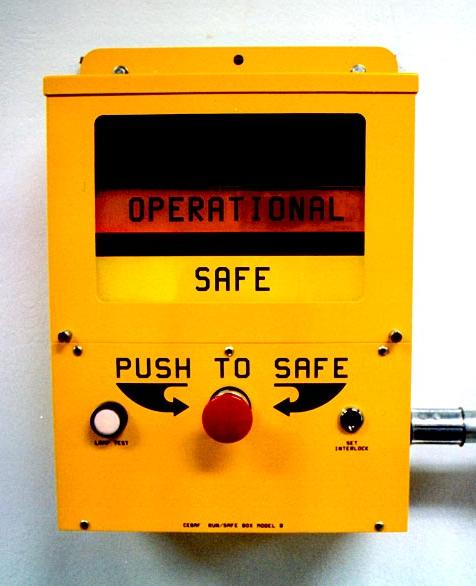
\includegraphics[angle=0,height=2.5in]{run-safe-box}\hspace{0.25in}
  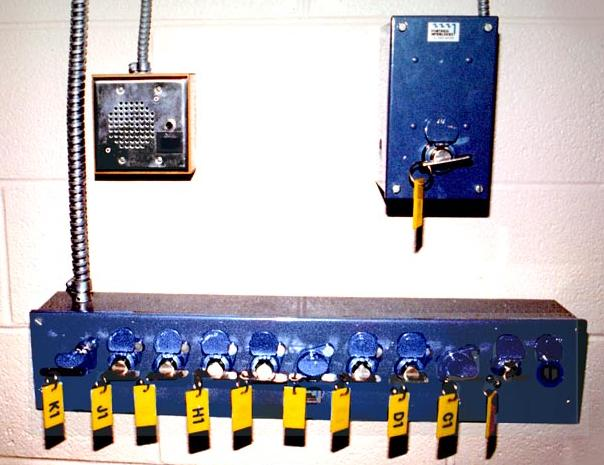
\includegraphics[angle=0,height=2.5in]{access-keys}
\end{center}
\caption[Introduction: Runs/Safe box, Access Keys]{Run/Safe box (left) 
  and Access Keys (right)}
\label{fig:run-safe-box}
\end{figure}

\begin{safetyen}{10}{10}
\section{Hall~A Access} 
\end{safetyen}

Access to Hall~A is governed by the ``Jefferson Lab Beam Containment
Policy and Implementation'' document~\cite{EHScebaf6310T2}.
%This document can be found in
%the Jefferson Lab ES\&H Manual (Section 6310, Appendix T2). 
Work in
designated radiation areas will be governed by the Jefferson Lab
RadCon Manual~\cite{RADCONcebaf}.  Access procedures during 
Research Operations depend on
the number of individuals who will be entering the hall and the length
of time they are expected to be there.  A controlled access is used
when a few individuals require entry for a short period of time. If
the hall must be open for an extended period and many people will
enter, then you should use the restricted access procedure instead of
the controlled access procedure.  Normally, when requesting a
controlled access, the hall will be in either the Beam Permit or RF
Permit State - for example, if the beam has been on or it could be
shortly.  If the hall is not already in the Controlled Access state
when you wish to access it, you must request a change to that state
from the Machine Control Center at extension 7050 and indicate that
you intend to make a Controlled Access. The MCC will then send an
Assigned Radiation Monitor to survey the hall. Before anyone enters
the hall, the ARM will carry out a radiation survey and post radiation
areas. Subsequent entry by individuals during the same Controlled
Access period does not require an ARM survey.

\begin{safetyen}{10}{10}
\subsection{Access Requirements}
\label{sec:access-req}
\end{safetyen}

  Normally only registered experimenters, authorized contractors or
sub-contractors and Jefferson Lab employees may enter experimental
areas. 
In addition, lab policy states that no one under eighteen years
of age is allowed access to the experimental halls.

\noindent{}In order to take part in Hall A operations 
  and get access into Hall A one has to
  fulfill at least the following Jefferson Lab safety 
  training\footnote{This list is valid by Dec,2003}%, consult ???}:  

 \newcounter{enumtmp}
 \newcounter{enumtmp1}
 \begin{list}{\arabic{enumtmp}.~}{\usecounter{enumtmp}\setlength{\itemsep}{-0.2cm}}    
    \item EH\&S orientation~\cite{EHScebaf};
    \item Radiation Worker I (RW-I) training~\cite{RWIcebaf};
    \item Oxygen Deficiency Hazard (ODH) training~\cite{ODHcebaf}.
    \setcounter{enumtmp1}{\value{enumtmp}}
 \end{list}
\noindent{}Additionally, one has to get training specific to
 Hall A operations. A part of this training is general
(independent on the experiment currently running):
 \begin{list}{\arabic{enumtmp}.~}{\usecounter{enumtmp}\setlength{\itemsep}{-0.2cm}}    
    \setcounter{enumtmp}{\value{enumtmp1}}
    \item Hall A safety awareness (``walkthrough'')~\cite{SAThalla}\footnote{Required
          for entering the Hall and for working in the counting house.
         For working in the counting house only, the training may be reduced
        to the appropriate part.};
    \item Hall A Radiation Work Permit (RWP) (read/sign)\footnote{Available in counting house,
          updated by Ed Folts}.
    \setcounter{enumtmp1}{\value{enumtmp}}
 \end{list}
\noindent{}In order to take part in shifts of a given experiment the following
  experiment-specific orientation is required\footnote{Available in counting house, 
   provided by the spokespeople of the experiment.}:
 \begin{list}{\arabic{enumtmp}.~}{\usecounter{enumtmp}\setlength{\itemsep}{-0.2cm}}    
    \setcounter{enumtmp}{\value{enumtmp1}}
    \item Conduct of Operations (COO) (read/sign);
    \item Experiment Safety Awareness Documents (ESAD) (read/sign);
    \item Radiation Safety Awareness Documents (RSAD) (read/sign).
 \end{list}
 
As exception, someone without training items 2(GERT~\cite{RWIcebaf} is still required
with a temporary TLD dosimeter),
3 and 4 can enter the hall with an escort. \\

 In addition to the above, undergraduate students must undergo a three
 month trial period. During this period they may work in the hall
 provided that:

\begin{itemize}
\item Their work in the hall is directly supervised by a hall
 authorized ``buddy'' (who CANNOT be an undergraduate)
\item Either a JLab staff member or a fully trained user has
 supervisory responsibility for and is fully cognizant of all their
 work
\item The person with supervisory responsibility has approved the
``buddy''.
\end{itemize}

\noindent{}After completion of the trial period undergraduates may be
approved for work in the halls under the standard guidelines. \\ 

\noindent{}Physics Division EH\&S personnel should be contacted to obtain
the current policy for conducting tours in the experimental areas.\\ 

\noindent{} More information on CEBAF operations and safety can be found in:
 \begin{list}{--}{\setlength{\itemsep}{-0.2cm}}
    \item Personnel Safety System (PSS) manual~\cite{PSScebaf};
    \item Accelerator Operations Directive~\cite{AODcebaf}.
 \end{list}


 \noindent{}Reading of this OSP is required for any involvement
 with the base equipment. 
 It is always referred to from ESAD (see item 7).


\begin{safetyen}{10}{10}
\subsection{Controlled Access Procedure} 
\end{safetyen}

To make a controlled access when the hall is in the controlled access
state, first contact the MCC. The MCC will unlock the first gate at
the entrance to the hall. Once inside, the MCC will release the master
key~\ref{fig:run-safe-box}. 
Remove the master key and insert it into the right-most slot of
the row of keys below it. Once the master key is in place, each person
wishing to gain access must remove a key from this row. The MCC will
then verify each person's name, which key he has, and check that each
person is wearing the proper dosimetry. This key-release procedure
allows the MCC to keep a ``count" of who has entered the hall. After
the procedure is complete, the MCC will unlock the second gate at the
entrance to the hall. Please note: only one of the entrance gates can
be open at a time while in the controlled access state.
 
When your work is completed and you are ready to exit, return to the
entrance gates and call MCC (7050) to notify them of your intention to leave.
 Once you have entered and closed the first gate, each person must
replace his key in the appropriate slot, otherwise the Personnel
Safety System will not allow the master key to be released. When the
master key is released, place it in its slot, and the MCC will unlock
the final gate. When you have exited the final gate, make sure it has
closed and locked behind you. If circumstances dictate, request that
the MCC return the hall to the beam permit state and that beam be
restored.  It is important to note that if you need to work in the HRS
shield house during the controlled access, you must go to the control
room in the MCC before the access and get a special key which allows
you to arm the run/safe box located in the shield house. The run/safe
box inside the shield house will drop from the operational position to
the safe position as soon as the door to the shield house
opens. Unless this box is rearmed with the special key, the beam
cannot run.

\begin{safetyen}{10}{10}
\subsection{Restricted Access Procedure} 
\end{safetyen}

Restricted Access is used when the hall will be open for an extended
period of time or a large group will enter to work. 
To drop the hall
to the Restricted Access state, first get approval from Run 
Coordinator\footnote{The Run Coordination is the immediate on-site
manager of the experiment and is appointed for a period from
several days to about two weeks.}
(if one is assigned for the given time period)
and Hall A Work Coordinator\footnote{Ed Folts, pager 584-7857},
then notify the MCC that you wish to
open the hall in the Restricted Access state. The MCC will drop the
hall status to Controlled Access and send an ARM to survey the
hall. Before anyone can enter the hall, the ARM will carry out a
radiation survey and post radiation areas.  The hall is placed in
Controlled Access during the survey to ensure that no one enters
before it has been completed. Upon completion of the survey and
posting of radiation areas, the ARM will leave the hall and notify the
MCC that they can drop the hall state to Restricted Access. With the
hall in the Restricted Access state, anyone with the appropriate
training may enter and work.  The key- release procedure is not
required.
 
To return the hall to Beam Permit from the Restricted Access state, a
full inspection must be carried out. This is begun by setting all
equipment to its operating state (following the Hall~A checklist) and
then clearing all workers out of the hall. Next, a request is made to
the MCC to arrange a sweep of the hall and to restore the Beam Permit
state. The MCC will send over an ARM and set the hall status to Sweep.
The ARM will then sweep the hall, verifying that everyone is
out. Following a successful sweep, the MCC can move the hall through
the Controlled Access and RF Permit states to the Beam Permit state.
While working in the hall you must observe all posted radiation areas.
Remember, work inside a radiation area requires that you obtain an
approved radiation permit. You must also observe the ``two-man" rule,
and pay attention to the alarms.

\begin{safetyen}{10}{10}
\subsection{The Hall A Safety Walk-through}
\end{safetyen}

In order to improve user awareness of the systems in the hall,
users are required to complete a self-guided safety walk-through
the experimental area. Information about the walk-through can be
found on the web~\cite{SAThalla}.
%\htmladdnormallinkfoot{}{\url{
%http://hallaweb.jlab.org/news/minutes/walkschd.html
%}}.
John LeRose is the JLab staff member responsible for the
administration of the Hall A safety walk-through.

Fig.~\ref{fig:asafe} shows the location of
many of the safety related items in Hall A while
Fig.~\ref{fig:aelec} shows the location of all the circuit
breaker boxes in the hall.

\begin{figure}
\begin{center}
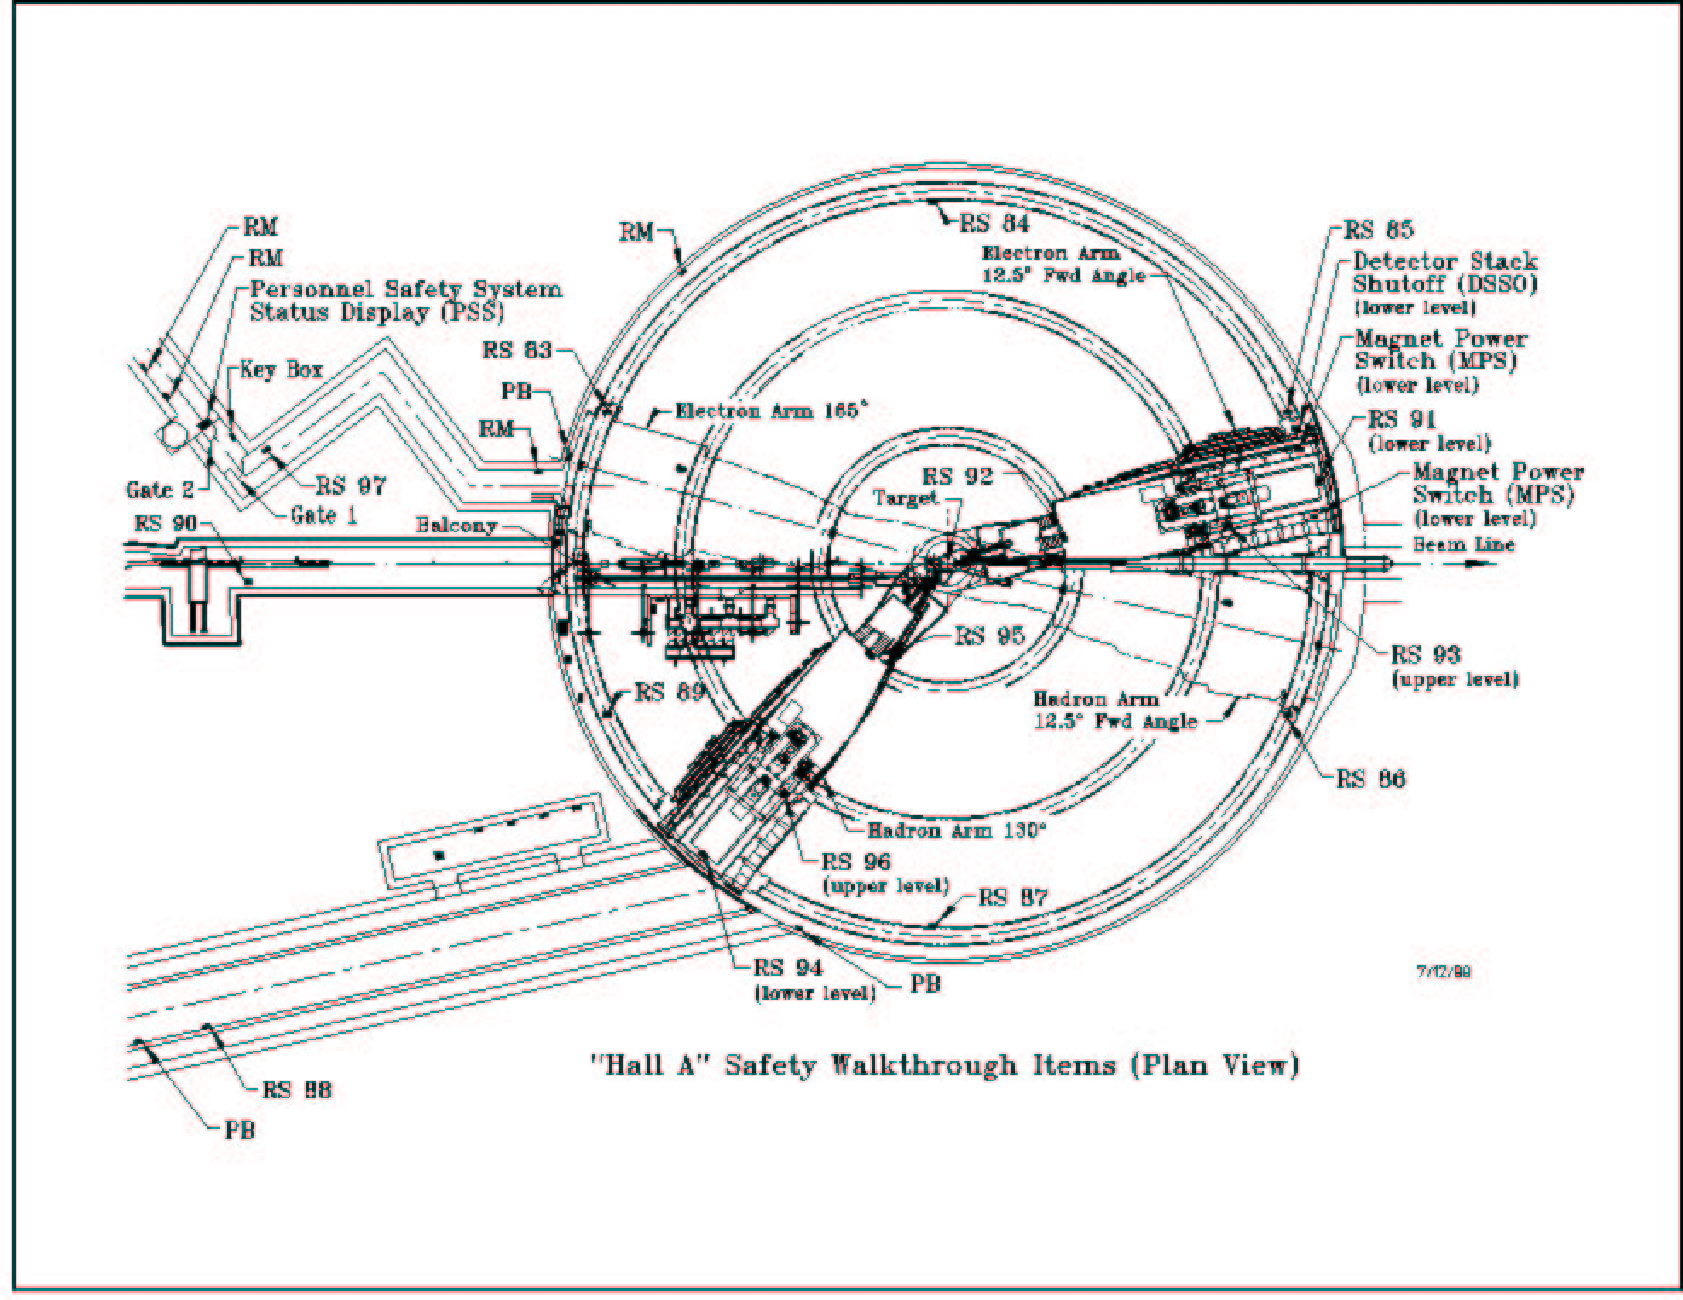
\includegraphics[angle=0,width=15cm]{asafe}
{\linespread{1.}
\caption[Introduction: Location of Hall Safety Items ]{Schematic
of the Hall A showing the location of various safety system
components. The abbreviations are: Radiation Monitor, RM, Run
Safe Box, RS, Fire Alarm Pull Box, PB. }
\label{fig:asafe}}
\end{center}
\end{figure}

\begin{figure}
\begin{center}
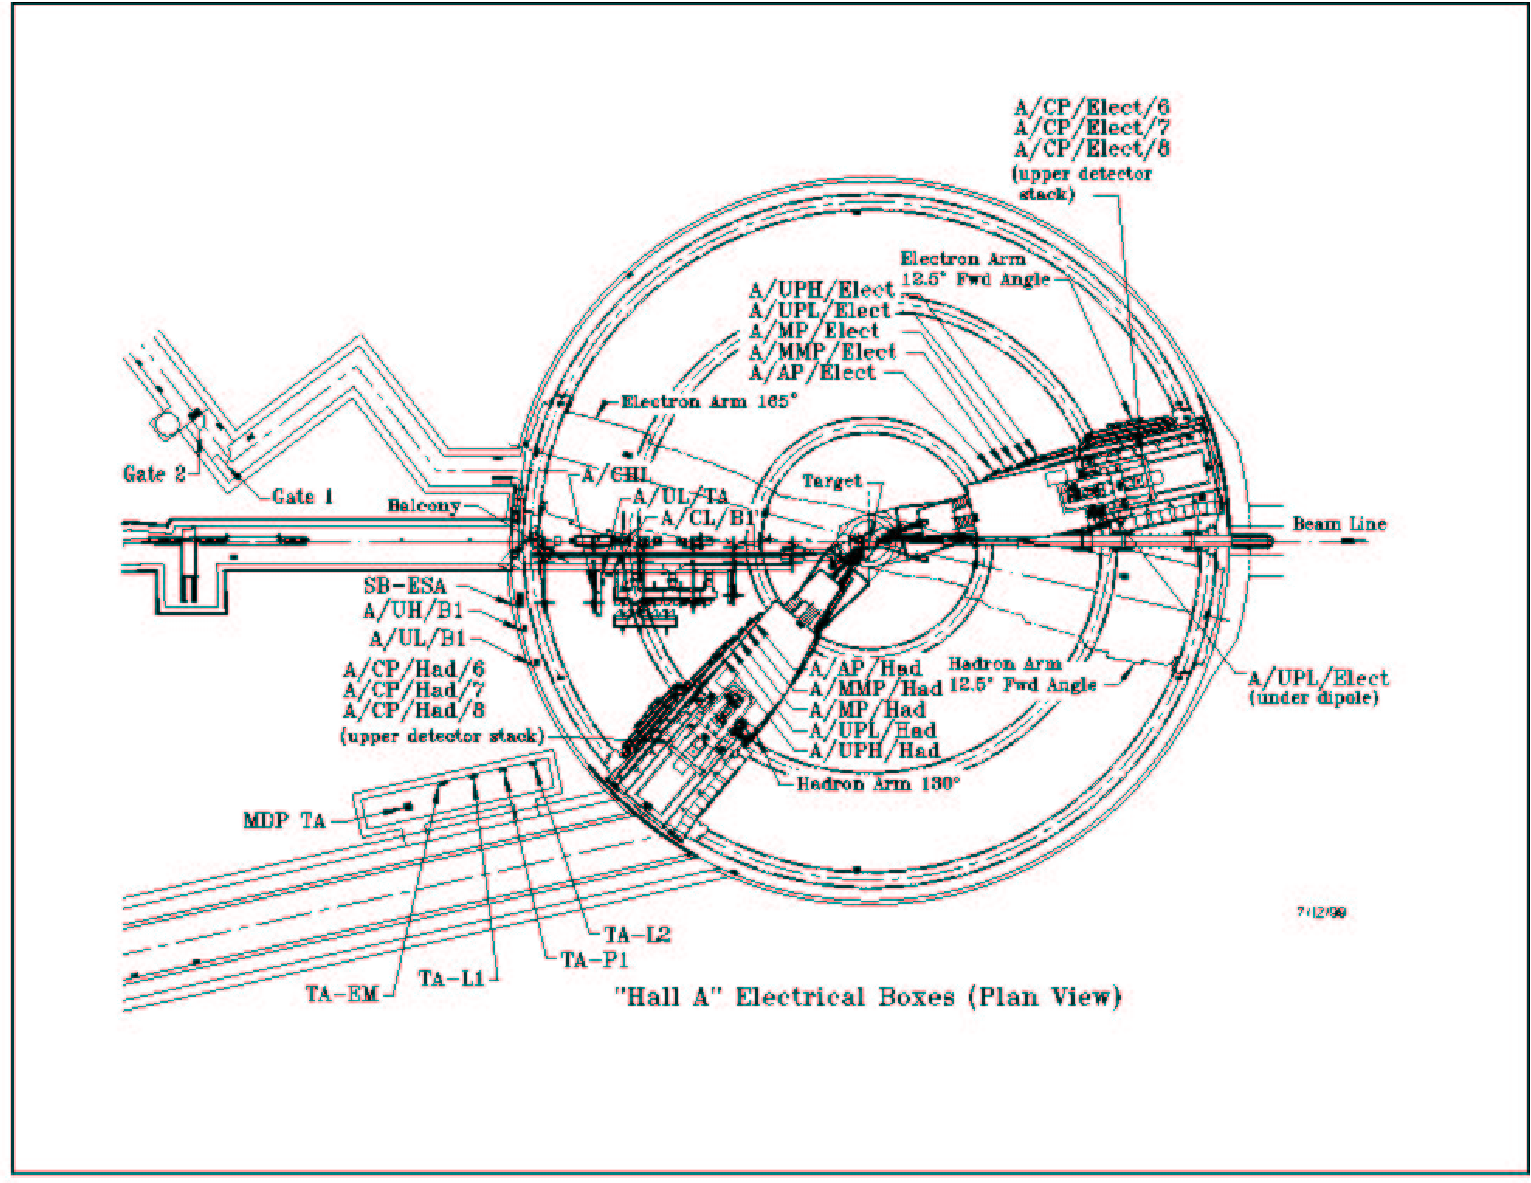
\includegraphics[angle=0,width=15cm]{aelec}
{\linespread{1.}
\caption[Introduction: Location of Circuit Breakers]{Schematic of
the Hall A showing the location of the circuit breaker panels.}
\label{fig:aelec}}
\end{center}
\end{figure}

% ===========  CVS info
% $Header: /group/halla/analysis/cvs/tex/osp/src/introduction/access.tex,v 1.1 2003/12/05 07:23:23 gen Exp $
% $Id: access.tex,v 1.1 2003/12/05 07:23:23 gen Exp $
% $Author: gen $
% $Date: 2003/12/05 07:23:23 $
% $Name:  $
% $Locker:  $
% $Log: access.tex,v $
% Revision 1.1  2003/12/05 07:23:23  gen
% Many modifications in the introduction, new pictures
%

